%\documentclass[licence,solution]{controle}
\documentclass[licence,10pts]{controle}
\matiere{Pratique du~C}
\genre{Fiche de TD 1}
\commentaire{Interpr\'eteur de commandes}
\usepackage[french]{babel}
\usepackage{epsfig}

\newcommand{\B}[1]{\overline{#1}}

%%%%%%%%%%%%%%%%%%%%%%%%%%%%%%%%%%%%%%%%%%%%%%%%%%%%%%%%%%%%%%%%%%%%%%%%%%%%%%
% graphismes
%

%\pssilent

\newlength{\longDSfig}

\def\normalDSfig{0.7}
\def\petiteDSfig{0.5}
\def\tinyDSfig{0.42}
\def\petiteXpixDSfig{0.9}
\def\smallDSfig{0.4}

\newcommand{\DSfig}[2]
{ \settowidth{\longDSfig}{\epsfig{figure=#1}}%
  \setlength{\longDSfig}{#2\longDSfig}%
  \ifthenelse{\lengthtest{\longDSfig > \linewidth}}%
    {\setlength{\longDSfig}{\linewidth}}%
    {\setlength{\longDSfig}{\longDSfig}}%
  \epsfig{figure=#1,width=\longDSfig}}

% the end

\begin{document}
\section{Introduction}
Cette note commence par expliciter quelques fondamentaux avant
d'aborder des notions relatives aux interpr\'eteurs de commandes.
\subsection{Structuration du syst\`eme de fichiers~: point de vue utilisateur}
 Un fichier est l'abstraction d'un flux lin\'eaire d'octets.
  \par
  Aucune information sur l'organisation de l'espace du support
  physique le stockant ne nous est utile \`a ce niveau d'abstraction.
  Pour manipuler les fichiers, il faut juste pouvoir les identifier
  par leurs caract\'eristiques~:
  \begin{itemize}
  \item nom, type, taille du fichier~;
  \item propri\'etaire du fichier (cf. sa repr\'esentation en
    section~\ref{sec:RepresentationUtilisateur})~;
  \item date de cr\'eation, date de derni\`ere modification~;
  \item protection~: qui a droit de le lire et de le manipuler~;
  \end{itemize}
  sans s'occuper de l'implantation de ces derni\`eres.

  \subsubsection{Droits d'acc\`es et masque binaire}
  Dans les syst\`emes d'exploitation d\'eriv\'es d'Unix, le codage des
  droits se fait sur~$9$ bits group\'es par~$3$ bits qui sont dans
  l'ordre~:
  \begin{enumerate}
  \item[r] le fichier est lisible par le propri\'etaire (\texttt{-}
    dans le cas contraire)~;
  \item[w] le fichier est modifiable par le propri\'etaire (\texttt{-}
    sinon)~;
  \item[x] le fichier est ex\'ecutable par le propri\'etaire
    (\texttt{-} sinon).
  \end{enumerate}
  Le groupe suivant de~$3$ bits reprend le m\^eme principe mais
  d\'efinit les droits pour les membres du groupe auquel appartient le
  propri\'etaire et le dernier groupe concerne les autres utilisateurs
  suivant le m\^eme sch\'ema.
  \par
  Ces droits sont cod\'es en un entier. Pour ce faire, on convient de
  la correspondance~:~${r=4}, {w=2}$ et~${x=1}$. Ainsi, les
  droits~rw-, correspondent \`a l'entier~(r=)4+(w=)2=6. Donc~rw-rw-rw-
  correspond \`a l'entier~$666$.
  \paragraph{Questions.}
  \begin{enumerate}
  \item \`A quels droits correspondent les entiers~$751, 521, 214$
    et~$150$~?
  \item Par quels entiers sont cod\'es les droits~rw-r-\,-r-\,-
    et~rwxr-xr-x~?
  \end{enumerate}
  \paragraph{Droits par d\'efaut.}
  Par ailleurs, \`a la cr\'eation d'un fichier, des droits d'acc\`es
  par d\'efaut sont donn\'es \`a ce fichier.  En standard, l'entier
  codant ces droits est~$666$ pour un fichier et~$777$ pour un
  r\'epertoire.
  \par
  La commande shell interne\footnote{Cette notion est d\'efinie dans
    la suite.} \texttt{umask} permet de d\'efinir la protection
  maximale que l'on donne au cours de la session aux nouveaux
  fichiers~; sa syntaxe est~: \verb?umask <octal>?.
  \par
  Les droits d'acc\`es sont d\'etermin\'es apr\`es l'op\'eration
  logique suivante~: d\'efaut ET (NON octal). Plus simplement et lorsque
  c'est possible, on part des droits par d\'efaut et on retranche le
  masque octal. Si ce n'est pas possible, on applique la r\`egle
  pr\'ec\'edente.
  \par
  Pour conna\^\i{}tre la valeur du masque courant, il suffit
  d'utiliser la commande umask sans arguments.
  \paragraph{Questions.}
  \begin{enumerate}
  \item \`A quels droits correspondent les masquages~$77$ et~$244$
    dans le cas d'un fichier et dans celui d'un r\'epertoire~?
    
  \item Quels masque faudrait-il appliquer afin d'obtenir pendant la
    session les droits~rw-rw-r-\,- \`a chaque cr\'eation de fichier dans
    le cas d'un fichier et dans celui d'un r\'epertoire~?
  \end{enumerate}

  \subsubsection{Organisation en graphe}%
  Ce type  de  repr\'esentation de la  communaut\'e  des  fichiers est
  assoupli en autorisant plusieurs ar\^etes  \`a pointer sur un m\^eme
  \'el\'ement et  en  faisant   pointer chaque r\'epertoire  sur   son
  pr\'ed\'ecesseur.
  \par
  \begin{tabular}{ll}
  \begin{minipage}{6cm}
    \vspace{-4cm} 
    On obtient ainsi un graphe qui permet~:
    \begin{itemize}
    \item   de   remonter    l'arborescence depuis   n'importe    quel
      r\'epertoire sans repartir syst\'ematiquement de la racine~;
    \item     de   permettre    l'acc\`es    depuis le    r\'epertoire
      \texttt{sedoglav} \`a  un fichier  r\'ef\'erenc\'e dans un autre
      r\'epertoire (lien symbolique cod\'e par un fichier).
    \end{itemize}
  Cette organisation  des fichiers est bas\'ee  sur un  type de fichier
  --- les r\'epertoires --- codant les ar\^etes constituant le graphe.
  Les r\'epertoires   \'etant  des  fichiers,   ils ont   les  m\^emes
  attributs (droits, etc).

  \end{minipage} 
  &
  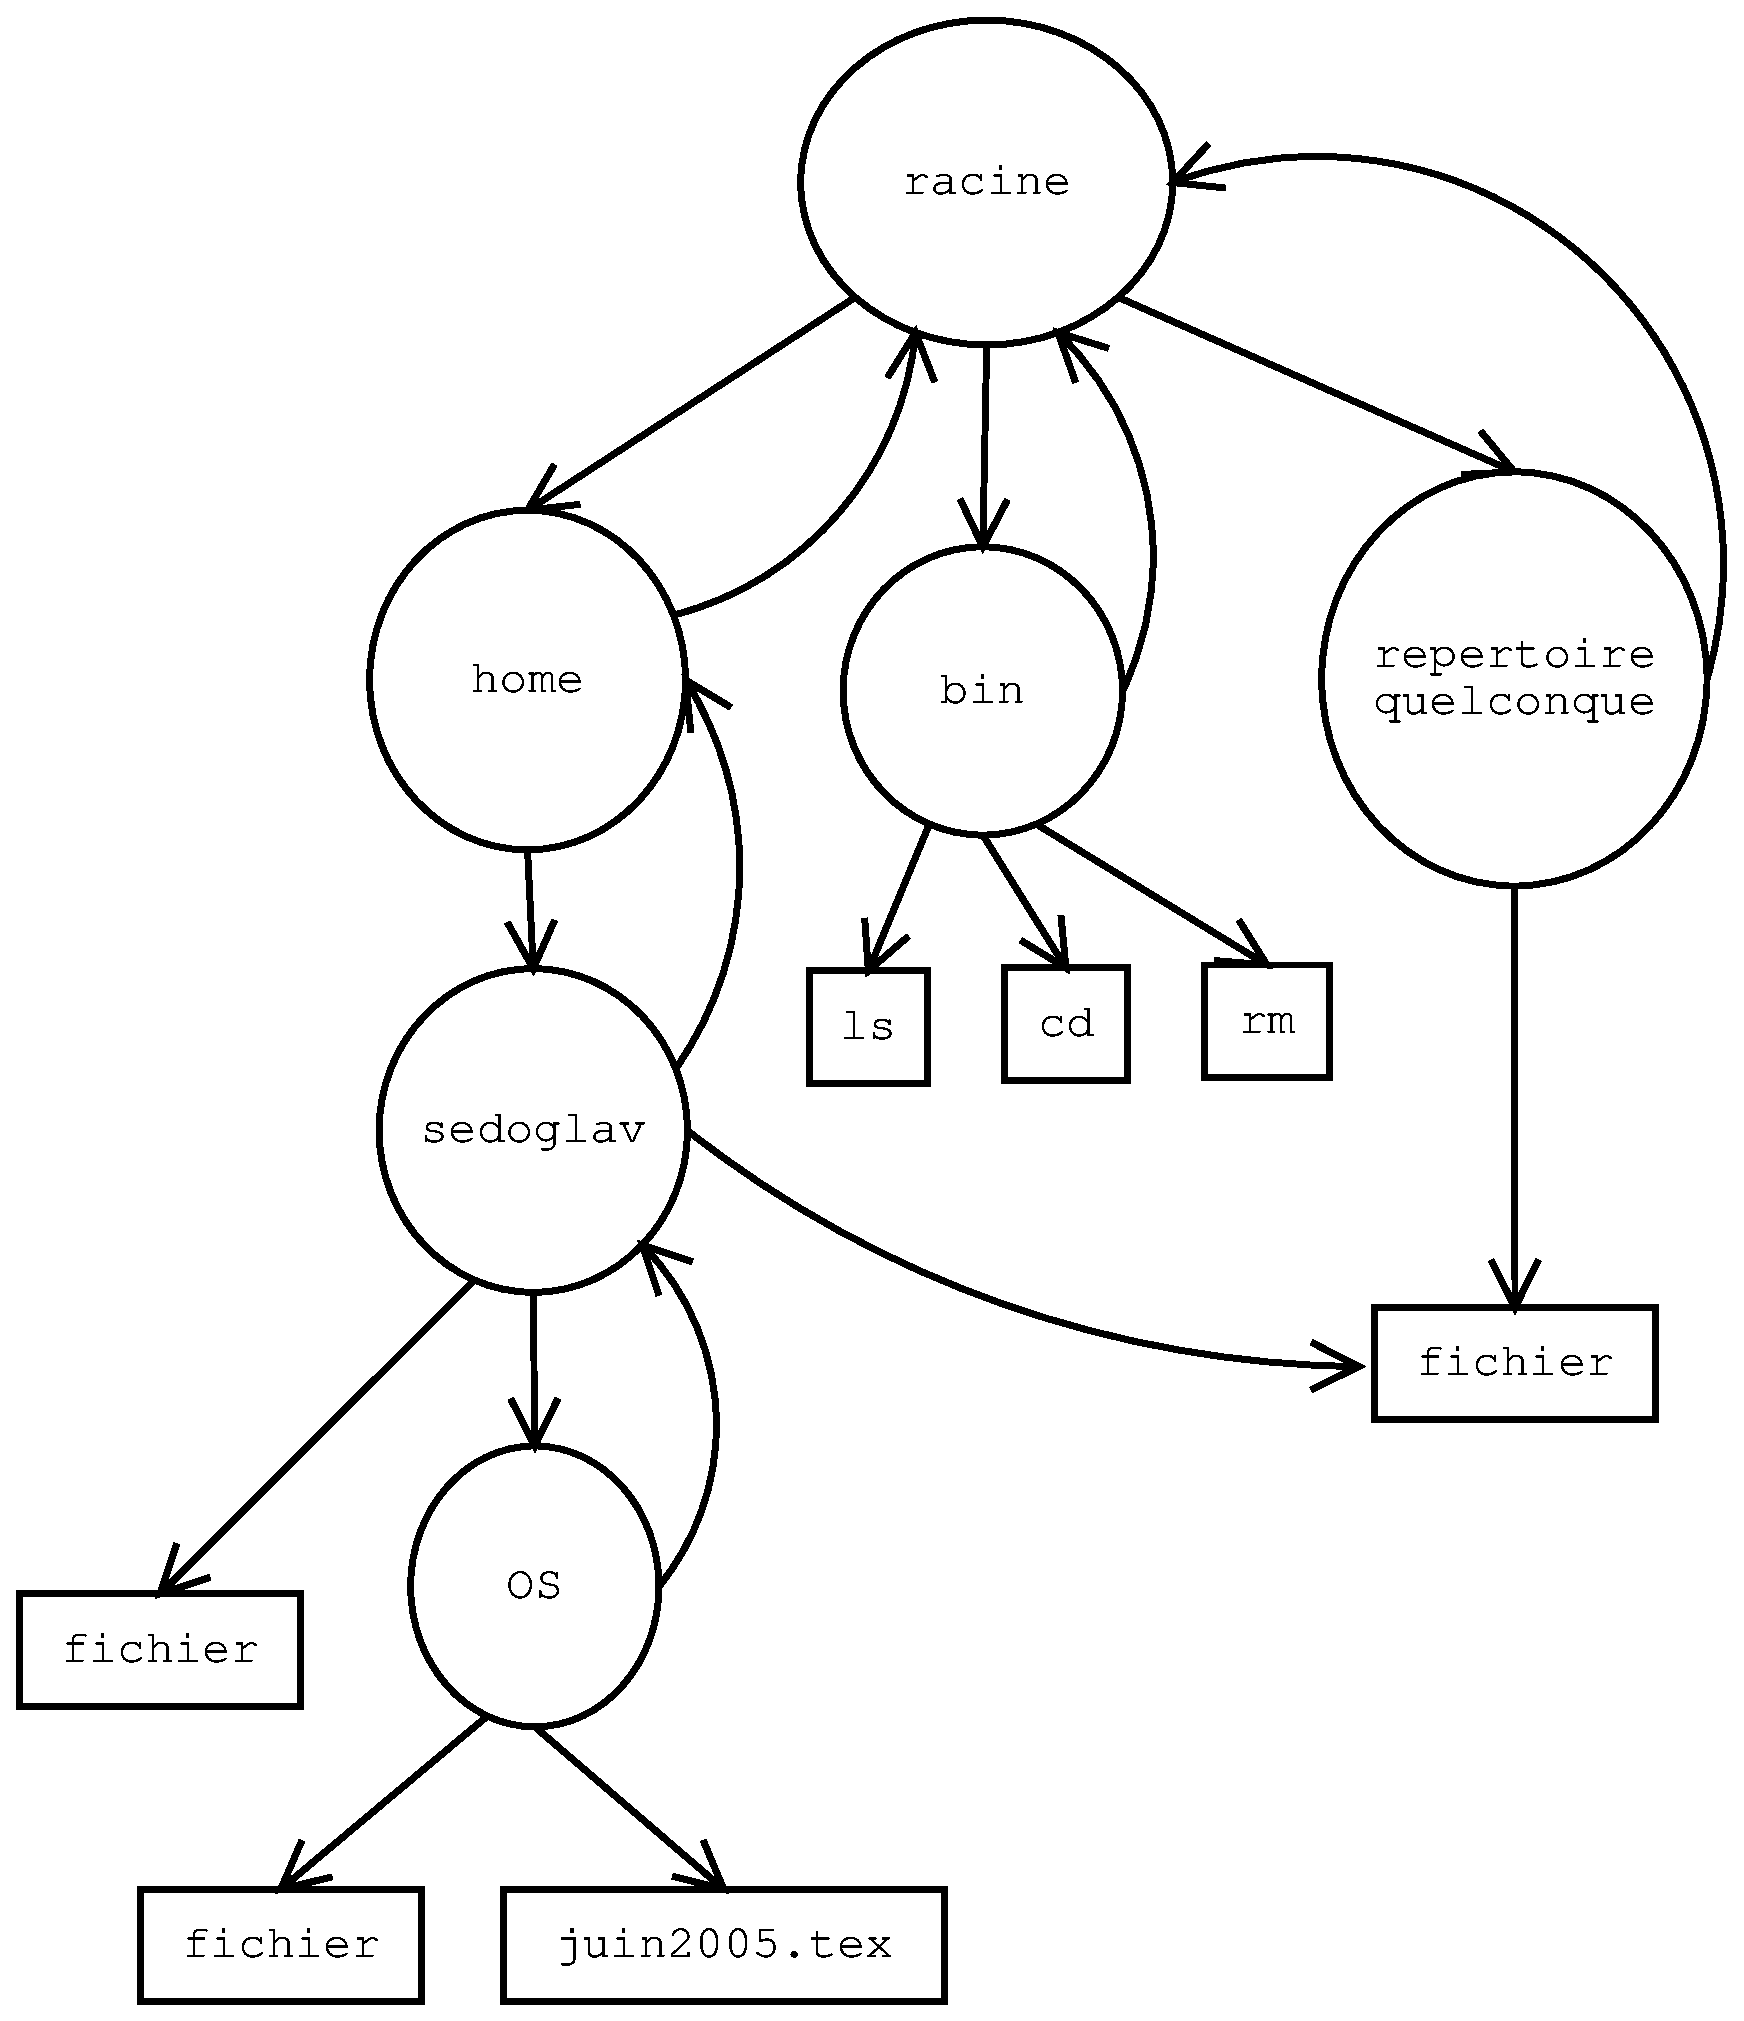
\includegraphics[scale=.16]{DAGFichier} 
\end{tabular}
\par
\subsection{Repr\'esentation de l'utilisateur par le syst\`eme}
\label{sec:RepresentationUtilisateur}
Tout utilisateur --- consid\'er\'e comme une entit\'e connue par le
syst\`eme d'exploitation --- est caract\'eris\'e par
  \begin{itemize}
  \item son \textit{login} i.e.\ le nom d'utilisateur~;
  \item son mot de passe~;
  \item un unique num\'ero d'identification (uid)~;
  \item un num\'ero de groupe d'utilisateur (guid) auquel il
    appartient~;
  \item un r\'epertoire i.e.\ son espace disque (\$HOME) dans
    l'arborescence du syst\`eme de fichiers~;
  \item le nom d'un programme d'interface entre l'utilisateur et le
    syst\`eme.
  \end{itemize}
  \par\medskip
  Par exemple pour les utilisateurs locaux (hors r\'eseaux), on trouve
  les informations dans le fichier \texttt{/etc/passwd}. L'information
  relative au superutilisateur dans ce fichier est~:
\begin{verbatim}
root:x:0:0:root:/root:/bin/bash
\end{verbatim}
\begin{question}
  Expliciter les informations contenues dans les lignes suivantes~:
\begin{verbatim}
manu:x:500:500:manu:/home_local/manu:/bin/csh
shutdown:x:6:0:shutdown:/sbin:/sbin/shutdown
\end{verbatim}
extraites d'un fichier \texttt{/etc/passwd}.
\end{question}
\section{Interpr\'eteurs de commandes~: les shells}%
Un \textit{shell} est un interpr\'eteur de commandes qui sert
d'interface entre l'utilisateur et le syst\`eme d'exploitation.
\par\medskip
Le shell peut \^etre utilis\'e suivant~$2$ modes~:
\begin{enumerate}
\item En mode interactif, il permet d'ex\'ecuter des programmes
  tout en offrant des \textit{op\'erateurs} destin\'es \`a combiner
  leurs actions.
\item En mode \textit{batch}, il offre un langage de programmation~:
  les instructions sont d\'efinies dans un \textit{script} que le
  shell interpr\`ete (pas de compilation).
\end{enumerate}
\par\medskip
Il existe plusieurs interpr\'eteurs de commandes qui sont~:
\begin{itemize}
\item d\'eriv\'es du Bourne shell (AT\&T) comme sh, ksh, bash, etc.~;
\item d\'eriv\'es du C shell (BSD) comme csh, tcsh, etc.
\end{itemize}
\par\medskip
Le shell pr\'esente une \textit{invite de commande} (disons~\%) qui
permet de saisir une commande du type~:
\begin{verbatim}
% <commande> [option(s) de la commande] [argument(s) de la commande]
\end{verbatim}
\par
Les commandes shell sont de~$2$ types~: interne et externe. 

\subsection{Commandes externes}
Ce type de commande provoque l'ex\'ecution d'un processus \`a partir
d'un fichier ex\'ecutable \'eponyme de la commande et se trouvant dans
l'arborescence du syst\`eme de fichiers (dans le r\'epertoire
\verb+/usr/bin+ par exemple).
\par
  L'outil fondamental est le manuel d'utilisation \texttt{man} et la
    premi\`ere chose  \`a  faire est de lire  l'aide  sur le manuel en
    utilisant la commande  \texttt{\% man man} dans votre interpr\'eteur
    de commandes favori.
    \begin{itemize}
  \item[\texttt{\% man -a mount}]  affiche  l'ensemble des  pages  d'aide
    contenant le mot mount. Entre autre~:
\begin{verbatim}
mount                (2)  - mount and unmount filesystems
mount                (8)  - mount a file system
\end{verbatim} 
  \item[\texttt{\% man  -S8   mount}] affiche  l'aide sur  \texttt{mount}
    issue de la section~$8$ du manuel.
  \end{itemize}
  On  peut aussi utiliser  l'utilitaire  \texttt{info} mais, bien  que
  plus \'evolu\'e (liens hypertext), il n'est pas forcement complet.
  
  Ceci fait les commandes shell n'auront plus de secrets pour vous~:

  \subsection{Les t\^aches de fond et le contr\^ole des processus}%
  Par d\'efaut, les shells attendent la fin de l'ex\'ecution d'une
  commande avant de permettre la saisie et l'ex\'ecution d'une autre.
  \par
  Pour d\'etruire une application dont le shell attend la terminaison,
  on utilise le raccourci clavier CTRL-C.  Pour interrompre sans
  d\'etruire une application, on utilise le raccourci clavier CTRL-Z.
  \par\medskip
  Les shells permettent aussi de lancer une application en
  \textit{t\^ache de fond} et ainsi l'ex\'ecution d'une autre (m\^eme
  si la premi\`ere n'est pas termin\'ee). Pour ce faire, on termine la
  commande par~\&.
  \paragraph{Les commandes externe ps et kill}%
  Un num\'ero identifiant est associ\'ee \`a chaque  processus.
  La commande externe \verb?ps? permet d'afficher les informations
  associ\'ees aux processus.
\begin{verbatim}
% ps -l
F S   UID   PID  PPID  C PRI  NI ADDR SZ WCHAN  TTY          TIME CMD
0 S  6013  2434  2426  0  75   0 -   954 rt_sig pts/1    00:00:00 csh
0 S  6013  2688  2434  0  69   0 -  3523 select pts/1    00:00:04 xemacs
0 R  6013  3061  2434  0  76   0 -   895 -      pts/1    00:00:00 ps
\end{verbatim}
  Les processus peuvent recevoir un signal envoy\'e par la commande
  externe \verb?kill -<Signal> <PID>?. Les principaux
  signaux sont~:
  \begin{center}
    \begin{tabular}{c|l}
      Signal & Signification \\\hline{}
      15     & terminaison de processus \\
      9      & destruction inconditionnelle de processus (CTRL-C)\\
      19     & suspension de processus (CTRL-Z)\\
      18     & reprise d'ex\'ecution d'un processus suspendu
    \end{tabular}
  \end{center}

\subsubsection{Expressions r\'eguli\`eres et m\'eta-caract\`eres}
Il s'agit d'expressions d\'ecrivant des r\`egles des propri\'et\'es de
cha\^\i{}nes de caract\`eres. Pour ce faire, on utilise en shell les
\textit{m\'etacaract\`eres}~:
  \begin{itemize}
  \item le point d'interrogation \texttt{?}\ correspond \`a n'importe
    quel caract\`ere (sauf EOL).  L'expression r\'eguli\`ere
    \texttt{b?l} repr\'esente les cha\^\i{}nes \textit{bal} et
    \textit{bol} et toutes les autres combinaisons comme
    \textit{bwl}~;
  \item la paire de crochet \texttt{[ ]} permet de sp\'ecifier plus
    restrictivement un ensemble de caract\`eres. L'expression
    r\'eguli\`ere \texttt{dupon[dt]} ne repr\'esente que les
    cha\^\i{}nes \textit{dupond} et \textit{dupont}. L'expression
    r\'eguli\`ere \texttt{dupon[d-t]} repr\'esente toutes les
    cha\^\i{}nes commen\c{c}ant par \textit{dupon} et se terminant par
    une lettre comprise entre \textit{d} et~\textit{t}. L'expression
    r\'eguli\`ere \texttt{dupon[\^{}dt]} repr\'esente toutes les
    cha\^\i{}nes commen\c{c}ant par \textit{dupon} et ne se terminant
    ni par un~\textit{d} ni par un~\textit{t}~;
    \item l'\'etoile \texttt{*} d\'esigne~$0,1$ ou plusieurs
      caract\`eres quelconques.  L'expression r\'eguli\`ere \texttt{*}
      repr\'esente toutes les cha\^\i{}nes.
  \end{itemize}
  Le pr\'efixe~$\backslash$ (antislash) transforme un
  m\'etacaract\`ere en caract\`ere.  \index{Shell!expression
    r\'eguli\`ere}
\begin{question}
  Utilisez la commande externe \texttt{ls} pour r\'ealiser l'exercice
  suivant.
\begin{enumerate} \item Lister les entr\'ees du r\'epertoire \texttt{/usr/bin} dont le
  nom commence par la lettre \texttt{m}. 
\item Lister les entr\'ees du r\'epertoire \texttt{/usr/bin} dont le
  nom commence par la lettre \texttt{m} et comporte exactement 3
  caract\`eres.  
\item Lister les entr\'ees du r\'epertoire \texttt{/usr/bin} dont le
  nom commence par la lettre \texttt{m} et comporte au moins 3
  caract\`eres.  
\item Lister les entr\'ees du r\'epertoire \texttt{/usr/bin} dont le
  nom commence par la lettre \texttt{m} et comporte une extension
  (suffixe suivant un \texttt{.}) non vide. 
\item Lister les entr\'ees du r\'epertoire \texttt{/usr/bin} dont le
  nom commence par la lettre \texttt{m} ou \texttt{j}. 
\item Lister les entr\'ees du r\'epertoire \texttt{/usr/bin} dont le
  nom commence par la lettre \texttt{m} et comporte une lettre
  majuscule. 
\item Lister les noms de fichiers  comportant une \'etoile \texttt{*}
\item Lister les entr\'ees du r\'epertoire \texttt{/usr/bin} dont le nom
  commence par la lettre \texttt{m} et ne comporte pas de lettre
  majuscule.
\end{enumerate}
\end{question}
\begin{solution}

\end{solution}
Il n'est pas possible de traiter la derni\`ere question avec la
commande \texttt{ls} et les m\'eta-caract\`eres. Il faudrait donc soit
pouvoir utiliser une autre commande, soit prendre le r\'esultat de 
\texttt{ls} pour finir de le traiter avec une autre commande.


  \subsection{Commandes internes et variables}%
  Toutes les commandes d'un shell ne sont pas externe. Par exemple, la
  commande \verb+cd+ qui permet de se d\'eplacer dans l'arborescence
  du syst\`eme de fichier n'est pas associ\'ee \`a un fichier
  ex\'ecutable du m\^eme nom.
  \par
  Autre exemple, la commande \texttt{setenv} ne correspond \`a aucun
  fichier ex\'ecutable mais est implant\'ee dans le code du shell.
  Cette commande est interne et permet d'afficher et de modifier des
  variables internes au shell~:
\begin{verbatim}
% setenv
USER=sedoglav
LOGNAME=sedoglav
HOME=/home/enseign/sedoglav
PATH=/usr/local/bin:/bin:/usr/bin:/usr/X11R6/bin:/usr1/bin:/usr/X11R6/bin
MAIL=/var/mail/sedoglav
SHELL=/bin/csh
HOSTTYPE=i586-linux
PWD=/home/enseign/sedoglav
GROUP=enseign
LANG=fr_FR
SYSFONT=lat0-16
TMP=/home/enseign/sedoglav/tmp
HOSTNAME=lxt2
\end{verbatim}
\index{Shell!variables}

  \paragraph{D\'efinition et affectation de variables~:} une variable est d\'efinie
  d\`es qu'elle est affect\'ee. En~sh, \verb+FOO="Bonjour le monde"+.
  En csh, on utilise \verb+% set FOO="Bonjour le monde"+
  \par
  La commande \texttt{echo}\footnote{externe sur mon syst\`eme mais
    qui peut \^etre interne sur d'autres.} permet d'afficher
  l'argument qui lui est fourni~:
\begin{verbatim}
% echo FOO
FOO
\end{verbatim}
Pour \'evaluer une variable, il faut pr\'efixer son nom par \$.
\begin{verbatim}
% echo $FOO
Bonjour le monde
\end{verbatim}
En~sh, la commande interne \texttt{export} \'etend la port\'e d'une
variable~: par d\'efaut, cette derni\`ere n'est connue que par le
processus courant~; apr\`es coup, cette variable est connue par tous
les processus fils. En~csh, on utilise~: \verb+% setenv FOO "Bonjour le monde"+.
 \paragraph{Quelques variables d'environnement.}%
  Les variables d\'efinies dans les fichiers \texttt{/etc/profile} et
  \texttt{\~{}/profile} sont cr\'e\'ees lors de l'ouverture d'une
  session.
  \par\medskip
  \begin{tabular}{ll}
    \$PATH & les r\'epertoires dans lesquels sont cherch\'es les ex\'ecutables  \\
      & des commandes externes \\ 
    \$HOME & votre r\'epertoire de travail \\
    \$TERM & le type de terminal \\
    \$PWD & le r\'epertoire courant \\
    \$DISPLAY & cette variable est utilis\'e par l'interface graphique \\
     & pour savoir o\`u se fait l'affichage\\
    \$PS1 & l'invite de commande
  \end{tabular}
  \par\medskip
  Ces variables d'environnement peuvent \^etre utilis\'ees depuis un
  programme~C (fonction getenv) lanc\'e depuis le shell.
  \paragraph{Variables pr\'ed\'efinies du Bourne shell}% 
  \begin{itemize}
  \item \verb|$#| : %$
    nombre d'arguments 
  \item \verb|$*|, \verb|$@| : tous les arguments de la commande 
  \item \verb|$0| : le nom de la commande
  \item \verb|$1| \`a \verb|$9| : les~$9$ premiers arguments de la
    commandes.
    \par 
    La commande interne \verb|shift| permet la renum\'erotation des
    arguments (\verb|$1| est perdu) et donc l'acc\`es aux arguments
    $\geq{}$10~; la variable~\verb+#+ est mis \`a jour.
  \item \verb|$$| : %$
    num\'ero du processus courant 
  \item \verb|$?| : toutes les commandes ont un code de retour --- cod\'e sur un octet ---
    (\emph{exit-status}) i.e.\ une valeur enti\`ere qui fournie une
    information sur le d\'eroulement de la commande.
    \begin{itemize}
    \item d\'eroulement normal $\Rightarrow{}$ \verb|$?| = 0 
    \item d\'eroulement anormal $\Rightarrow{}$ \verb|$?| $\neq$ 0 
    \end{itemize}
  \item nous verrons comment renvoyer en~C le code de retour.
  \end{itemize}
  \paragraph{Typage.}%
  Dans un shell, \textbf{tout n'est que cha\^\i{}ne de caract\`eres}.
  \par\smallskip
  Chaque commande est une cha\^\i{}ne que le shell \'evalue. On peut
  influer sur cette \'evaluation gr\^ace aux d\'elimiteurs suivants~:
  \begin{itemize}
  \item les quotes \verb?' '? bloquent l'\'evaluation~;
  \item les guillemets \verb?" "? forment une cha\^\i{}ne apr\`es
    \'evaluation des composantes~;
  \item les backquotes \verb?` `? forment une cha\^\i{}ne \'evalu\'ee
    comme une commande.
  \end{itemize}
\begin{verbatim}
% echo '$FOO'
$FOO
% echo "echo '$FOO'"
echo 'Bonjour le monde'
% set BAR="n\'importe quoi"
% echo $BAR
n\'importe quoi
% set BAR=`n\'importe quoi`
n'importe: Command not found.                
\end{verbatim}
  \subparagraph{Cons\'equence sur la manipulation d'entiers.}%
  Pour utiliser l'arithm\'etique de base, il faut \'evaluer des
  cha\^\i{}nes de caract\`eres codant des expressions arithm\'etiques
  gr\^ace \`a la commande externe \texttt{expr}~:
\begin{verbatim}
% set i=12;set i=`expr $i + 1`
% echo $i $?
13 0
% expr 2 \* 2
4
\end{verbatim}
  Le code de retour de la commande \verb|expr|~:
  \begin{itemize}
  \item[0] si le r\'esultat est diff\'erent de~$0$ ;
  \item[1] si le r\'esultat est \'egal \`a~$0$ ;
  \item[2] si un argument est non num\'erique.
  \end{itemize}

  \subsection{Les op\'erateurs de composition de commandes dans un shell}%
  Le point virgule~; permet de s\'eparer des commandes.
  \par\medskip
  L'esperluette~\& permet de lancer une commande en t\^ache de fond.
  \par\medskip
  Une ligne de commande entre parenth\`ese est ex\'ecut\'ee dans un
  autre shell lanc\'e par le shell courant.
  \par\medskip
  Le shell dispose de~$2$ op\'erateurs conditionnels~:
  \begin{itemize}
  \item[\verb?cmd1 \&\& cmd2?~:] cmd2 est ex\'ecuter ssi cmd1
    retourne~0~;
  \item[\verb?cmd1 $||$ cmd2?~:] cmd2 est ex\'ecuter ssi cmd1 retourne
    un code non nul.
  \end{itemize}

  \paragraph{Redirection de flux.}
  Par d\'efaut, chaque processus poss\`ede~$3$ fichiers d'entr\'ee-sortie~:
  \begin{itemize}
  \item[stdin~0] est l'entr\'ee standard (par d\'efaut, le clavier)~:
  \item[stdout~1] est la sortie standard (par d\'efaut, l'\'ecran)~:
  \item[stderr~2] est la sortie des erreurs (par d\'efaut, l'\'ecran).
  \end{itemize}
  \par\medskip
  Ces flux peuvent \^etre redirig\'es~:
  \begin{itemize}
  \item[$<$] entr\'ee standard \`a partir d'un fichier~;
  \item[$>$] sortie standard dans un fichier (cr\'eation ou \'ecrasement)~;
  \item[$>>$] sortie standard dans un fichier (cr\'eation ou ajout)~;
  \item[]\verb$<<EOF texte EOF$ insertion de texte dans l'entr\'ee standard~;
  \item[$|$] tube de communication~;
  \item[$2>$] sortie des erreurs dans un fichier (bash uniquement)~;
  \item[$>$\&] sortie standard et erreur dans un fichier.
  \end{itemize}
  \begin{question}
    Sachant que la commande \verb+sleep+ d\'ecompte un temps donn\'e
    en argument sans rien faire, tentez de d\'eterminez \`a l'avance
    le comportement des instructions suivantes~:
\begin{verbatim}
sleep 5 ; echo A
echo A ; sleep 5
sleep 5 & echo A
echo A & sleep 5
(echo A ; sleep 5) &
echo A ; sleep 5 ; echo B
echo A ; sleep 5 & echo B
(echo A ; sleep 5 ) & echo B
echo A ; (sleep 5 & echo B)
echo A ; (sleep 5 ; echo B) &
sleep 5 & echo A ; ( sleep 5 ; echo B)
sleep 5 & echo A & ( sleep 5 ; echo B)
sleep 5 & echo A & ( sleep 5 & echo B) &
sleep 5 & echo A & ( sleep 5 ; echo B) &
\end{verbatim}
  \end{question}
  \begin{question}%[Exemple d'utilisation de redirection.]
  Le nom de la
  commande externe \verb+grep+ vient de "global regular expressions
  parsing" ("analyse d'expressions r\'eguli\`eres globales").  Elle
  permet de rechercher une expression r\'eguli\`ere dans chaque ligne
  d'un ou de plusieurs fichiers pass\'es en param\`etres (ou dans
  chaque ligne de l'entr\'ee standard) et affiche ces lignes sur la
  sortie standard.
  
  Que devrait retourner la ligne de commande suivante~:
\begin{verbatim}
% grep a << separateur
> Alexandre
> Virginie
> separateur
\end{verbatim}
  \textbf{Indication.} La commande grep re\c{c}oit le texte situ\'e
  entre les deux occurrences du s\'eparateur.
  \end{question}
  



\subsubsection{La notion de filtre}

Une ligne de commande qui peut recevoir des donn\'ees par
l'interm\'ediaire de son entr\'ee standard et fournir des r\'esultats
\`a sa sortie standard est appel\'ee un filtre.

Les filtres pr\'esentent le gros avantage de pouvoir \^etre
"branch\'es" les uns \`a la suite des autres~: en redirigeant la
sortie standard d'un filtre sur l'entr\'ee standard d'un autre, on
peut r\'ealiser un nouveau filtre.

\begin{question}[Redirection]
Dans cet exercice, nous allons utiliser les redirections coupl\'ees \`a
d'autres commandes~:  \texttt{grep}, \texttt{cut},


\texttt{tr} et \texttt{sort}.




\begin{enumerate}
%%Interet le pipe
\item Listez les entr\'ees du r\'epertoire \texttt{/usr/bin} dont le nom
  commence par la lettre \texttt{m} et comporte au moins une lettre
  majuscule ! (Avec la commande \texttt{grep}).
%%Interet grep -v et tjs le pipe
\item En vous servant de la question pr\'ec\'edente, r\'ealisez la derni\`ere
  question de l'exercice 1.
\end{enumerate}
\end{question}

\begin{question}
La commande \texttt{ls -l} permet d'afficher l'ensemble des informations
sur les fichiers d'un r\'epertoire.
\begin{verbatim}
total 104K
-rw-r--r--  1 dumont  west  234 Sep 28 11:33 td1.aux
-rw-r--r--  1 dumont  west 6.2K Sep 28 11:33 td1.dvi
-rw-r--r--  1 dumont  west 7.1K Sep 28 11:33 td1.log
-rw-r--r--  1 dumont  west 3.7K Sep 28 12:01 td1.tex
\end{verbatim}
\begin{enumerate}
%%Interet pipe + cut
\item Listez uniquement les propri\'et\'es des fichiers se trouvant
  dans un r\'epertoire (on se servira de l'exemple ci-dessus).
%ls -l | cut -f1 -d' '
\item M\^eme question mais en listant cette fois-ci, le nom du
  propri\'etaire, le mois de la derni\`ere modification et le nom de
  ces fichiers. Attention il y a un pi\`ege !
%ls -l | tr -s ' ' | cut -f3,6,9 -d' ' -s
\item Sauvegardez le r\'esultat de la derni\`ere commande dans un
  fichier. Triez suivant le nom des propri\'etaires et le nom du
  fichier (dans l'ordre alphab\'etique) et sauvegardez le r\'esultat
  \`a nouveau dans ce m\^eme fichier.
  Recommencez en vous passant de fichier auxiliaire.
\end{enumerate}
\end{question}

\section{Annexe}
Les descriptions des commandes dans cette annexe sont sommaires.
Utilisez le manuel en ligne pour avoir une description compl\`ete.
\paragraph{cut}
 Cette commande permet de supprimer une partie des lignes d'un ou de plusieurs fichiers, ou de l'entr\'ee standard. Sa syntaxe est~:
\begin{verbatim}
% cut -cliste [fichier ...]
% cut -fliste [-ddelimiteur] [fichier ...]
\end{verbatim}
L'option
\begin{itemize}
\item[-c] ne retient sur chaque ligne que les caract\`eres situ\'es
  \`a une position donn\'ee par liste. Par exemple, l'option -c1-50 ne
  garde que les 50 premiers caract\`eres de chaque ligne.
\item[-f] ne retient qu'une liste de champs (s\'epar\'es soit par des
  tabulations, soit par un d\'elimiteur sp\'ecifi\'e par l'option -d).
  Par exemple, l'option -f1,3-5 conduira la commande \`a ne garder que
  les champs num\'eros 1, 3, 4 et 5 de chaque ligne.
\end{itemize}
\paragraph{tr}
 Cette commande permet la "traduction" de caract\`eres provenant de l'entr\'ee standard. Sa syntaxe est~:
\begin{verbatim}
% tr -s|-d string
\end{verbatim}
L'option
\begin{itemize}
\item[-s] \'elimine les r\'ep\'etitions des caract\`eres composant la
  cha\^\i{}ne de caract\`eres staring, en n'en laissant qu'un \`a chaque
  fois.
\item[-d] supprime toutes les occurrences des caract\`eres composant
  la cha\^\i{}ne de caract\`eres string.
\end{itemize}
\paragraph{sort}
Cette commande lit un ou plusieurs fichiers ou l'entr\'ee standard, et
affiche les diff\'erentes lignes, tri\'ees sur un ou plusieurs champs
selon l'ordre lexicographique. Les s\'eparateurs de deux champs sont
l'espace et la tabulation. Sa syntaxe est~:
\begin{verbatim}
% sort -k clef -u 
\end{verbatim}
L'option
\begin{itemize}
\item[-k] permet d'indiquer les champs \`a prendre en compte pour le
  tri. L'argument clef doit \^etre \'ecrit sous la forme
  premier\_champ[,dernier\_champ] la partie entre crochets \'etant
  optionnelle. Si cette partie est absente, cela signifie que le tri
  prend en compte tous les champs \'a partir du champ de num\'ero
  premier\_champ.
\item[-u] permet l'affichage d'un seul exemplaire des lignes
  identiques.
\end{itemize}
\end{document}
\begin{question}
  Nous allons illustrer la commande \texttt{find} ainsi que certains
  points du cours.
\begin{enumerate}
\item Que fait la  commande \verb?ps aux | grep $USER?
\item Que fait la  commande \verb?cat /etc/passwd | cut -d: -f1 | sort > ~/res?
%%Interet find et la substitution des meta caract\`eres
\item Lister tous les fichiers de votre r\'epertoire personnel et de ces
  sous r\'epertoires qui commence par la lettre \texttt{m}. Attention \`a la
  substitution des m\'eta-caract\`eres.
\item Que fait la  commande \verb?find . -name tmp -type d ! -empty?
\item Que fait la  commande \verb?find /usr/include -name ``*a*b*'' -exec ls -l?
\end{enumerate}
\end{question}

%%%%%%%%%%%%%%%%%%%%% PART 3
\begin{itemize}
\item Le shell ne conna\^\i{}t que les cha\^\i{}nes de caract\`eres ; 
\item Les valeurs enti\`eres sont stock\'ees comme des cha\^\i{}nes de
  caract\`eres ; 
\item Affectation : \texttt{nom-var=<chaine>} La variable \texttt{nom-var}
  re�oit la valeur de la cha\^\i{}ne de caract\`eres ; 
\item Attention, pas d'espace s\'eparateur autour du \texttt{=}
\item La valeur de la variable de nom \texttt{nom-var} est d\'esign\'ee
  par \texttt{nom-var}. L'interpr\'eteur/le shell substitue \`a chaque
  occurrence de \texttt{nom-var} la valeur (cha\^\i{}ne de caract\`eres)
  de la variable identifi\'ee par \texttt{nom-var}.
\item Exemples : 
\begin{verbatim}
% a="hello"
% b="Unix"
% c=a 
% d=b 
% echo $a $b $c $d
hello Unix a b       

% a=pwd
% b=`$a`
% echo $a $b
pwd /home/phm 
 
% a=`ls`
% echo $a
TP1 sujet.ps sujet.tex  

% `ls`
sh: TP1: command not found     

% date
Sun Sep 27 00:04:23 CEST 1998      
% `date`
sh: Sun: command not found
\end{verbatim}
\end{itemize}






